\chapter{ОбЧРК в системе с одной передающей и одной приемной антенной}
\section{Модель системы}
В данном разделе будет рассмотрена модель системы ОбЧРК. Была рассмотрена система передачи с воздействием канала. Канал в физическом смысле полагается как компоненты многолучевого распространения между передатчиком и приемником\cite{}. Так же канал может быть описан как свертка между переданным сигналом и некоторой импульсной характеристикой. В таком случае поступивший на вход приемника сигнал может быть описан следующим образом \eqref{siso_1}, где $y$ является вектором поступивших на вход приемника данных, $x$ это вектор переданных с выхода передатчика данных и $H$ это матрица свертки между входными данными и некоторой импульсной характеристикой. При этом переданный с выхода передатчика сигнал может быть связан с передаваемыми символами при помощи модели $PARATUCK2$ и ее двумя формами записи в векторизированной форме \eqref{siso_2}\eqref{siso_3}\cite{Book21}. 
\begin{align}
\mathbf{y}=\mathbf{Hx}
\label{siso_1}
\end{align}
\begin{align*}
\mathbf{y,x}\in\compl^{T\times 1}
\mathbf{H}\in\compl^{T\times T}
\end{align*}
\begin{align}
\mathbf{x}=\mathcal{X}_{[3]}=vec(\mathcal{X})=\mathbf{\Omega}_1 vec(\mathbf{S})
\label{siso_2}
\end{align}
\begin{align*}
\mathbf{\Omega}_1 \in \compl^{T\times T_s \cdot F}
\end{align*}
\begin{align}
\mathbf{\Omega}_1=(\mathbf{C}^{[b]T}\diamond \mathbf{C}^{[a]T})^T \diamond (\mathbf{b^T \otimes a}) \
\end{align}
\begin{align}
\mathcal{X}_{:,:,i}=\mathbf{a}\cdot diag(\mathbf{C}^{[a]}_{:,i})\cdot \mathbf{S} \cdot diag(\mathbf{C}^{[b]}_{:,i}) \cdot \mathbf{b} \label{siso_3}
\end{align}
Переданные данные могут быть сгенерированы при помощи модели $PARATUCK2$ третьего порядка в векторизованной форме или развертке третьего измерения. В таком случае матрица символов передаваемых при помощи системы передачи ОбЧРК будет записана как матрица основа $\mathbf{S}$ в модели $PARATUCK2$\cite{Book6}\eqref{siso_4}\eqref{siso_5}. Таким образом можно без изменений внести все символы в систему передачи. 

Каждый столбец в $\Camat$ матрице соответствует определенной поднесущей частоте для модуляции. Таким образом матрица $\Camat$ конструируется как значения поднесущих частот в каждом из столбцов. Таким образом матрица $\Camat$ может быть записана следующим образом \eqref{siso_1}.
 \begin{align}
 c^{[a]}_{t,f}=e^{-j2\pi\cdot(t\cdot f)/T_s} \label{siso_4}
 \end{align}
\begin{align}
\mathbf{C}^{[a]}=\begin{bmatrix}
e^{-j2\pi\cdot 0}& e^{-j2\pi\cdot 0}& \cdots & e^{-j2\pi\cdot 0} \\
e^{-j2\pi\cdot 0}& e^{-j2\pi\cdot 1/T_s}& \cdots &e^{-j2\pi\cdot F/T_s} \\
e^{-j2\pi\cdot 0}& e^{-j2\pi\cdot 2/T_s}& \cdots &e^{-j2\pi\cdot 2F/T_s} \\
&&\vdots \\
e^{-j2\pi\cdot 0}& e^{-j2\pi\cdot T/T_s}& \cdots & e^{-j2\pi\cdot T\cdot F /T_s} \\
\end{bmatrix} \label{siso_5}
\end{align}
Каждый столбец матрицы $\Cbmat$ определяет функцию фильтрации во временной области для заданного блока данных. Столбцы являются сдвинутыми версиями первого столбца. Сдвиг между соседними столбцами равен $T/T_s$\eqref{siso_7}. Элементы в столбце определяются по следующему выражению \eqref{siso_6}\cite{Book12}. При конструировании матрицы $\Cbmat$ задается коэффициент перекрытия $\alpha$.
\begin{align}
\begin{matrix}
u(t) &=& \left\{ \begin{matrix} 
\frac{1-\alpha +4\alpha/\pi}{\sqrt{T}}& if& t=0\\
\frac{\alpha}{\sqrt{2T}}[(1+\frac{2}{\pi})sin(\frac{\pi}{4\alpha})+(1-\frac{2}{\pi})cos(\frac{\pi}{4\alpha})] & if &t= \pm T/4\alpha\\
\frac{1}{\frac{t\pi}{\sqrt{T}}(1-\frac{4*\alpha t}{T})^2}(sin(\frac{\pi t (1-\alpha)}{T})+\frac{4\alpha t}{T} cos(\frac{\pi t (1+ \alpha)}{T}) ) &otherwise \\
\end{matrix} \right.
\end{matrix}\label{siso_6}
\end{align}
\begin{align}
\mathbf{C}^{[b]}=\begin{bmatrix}
\mathbf{u}_{0}& \mathbf{u}_{1}& \cdots &\mathbf{u}_{T_s}\\
\end{bmatrix} \label{siso_7}
\end{align}
Матрица $\Bmat$ при моделировании ОбЧРК становится столбцом $\bmat$ и в физическом смысле соответствует изменению по амплитуде между символами на различных временных позициях\cite{Book34}. Поскольку мы рассматриваем линейную независимую от времени систему то все значения в столбце равны единице. Кроме того таким образом можно выразить различные взвешивающие коэффициенты позволяющие не передавать символы по определенным временным позициям\eqref{siso_8}.
\begin{align}
\mathbf{b}=\mathbf{1}_{T_s\times 1} \label{siso_8}
\end{align}
\begin{align}
\mathbf{b}\in \real^{T_s\times 1} \label{siso_9}
\end{align}
Матрица $\Amat$ при моделировании GFDM становится строкой $\amat$ и в физическом смысле соответствует коэффициентам передачи для каждой поднесущей в течении одного блока передачи. В данной работе будет рассмотрена система где значения а могут быть структурированы двумя образами\eqref{siso_10}. В первом случае строка а имеет все единичные значения. Во втором случае величины в строке а могут быть распределены случайным образом между значениями $1$ и $0$. Так же при помощи строки $\amat$ может быть   аппроксимировано влияние канала. Однако точность такой аппроксимации мала.
\begin{align}
\mathbf{a}=\mathbf{1}_{1\times F} \label{siso_10}
\end{align}
\begin{align}
\mathbf{a}\in \compl^{1\times F} \label{siso_11}
\end{align}
Определив указанным образом соответствующие матрицы, сигнал на выходе передатчика может быть определен при помощи одного из последующих выражений \eqref{siso_13} \eqref{siso_14}. При этом модель системы ОбЧРК может быть совпадает с тензорной моделью $PARATUCK2$.
\begin{align}
\mathbf{x}^T=\mathbf{a}\cdot (\mathbf{C}^{[a]T} \odot (\mathbf{S}\cdot (\mathbf{C}^{[b]}\diamond \mathbf{b}^T)^T)) \label{siso_12}
\end{align}
\begin{align}
\mathbf{x}=((\mathbf{a}\diamond \mathbf{C}^{[a]})^T \cdot \mathbf{S}) \odot \mathbf{C}^{[b]} \mathbf{b}) \label{siso_13}
\end{align}
\begin{align}
\mathbf{x}=((\mathbf{b}^T\diamond \mathbf{C}^{[b]})^T \cdot \mathbf{S}^T) \odot \mathbf{C}^{[a]T} \mathbf{a}^T) \label{siso_14}
\end{align}
\begin{align*}
\mathbf{x} \in \compl^{T\times 1 }
\mathbf{a} \in \compl^{1\times F}
\mathbf{C}^{[a]} \in \compl^{T\times  F}
\end{align*}
\begin{align*}
\mathbf{C}^{[b]} \in \compl^{T \times T_s}
\mathbf{b} \in \compl^{T_s\times 1}
\mathcal{S} \in \compl^{F\times T_s }
\end{align*}
\section{Полу-слепой приемник для оценки канала с памятью}
\subsection{Приближенное устранение влияния канала}
В данной секции будет описан метод приближенного вычисления влияния на принятый сигнал\eqref{siso_a_1}\eqref{siso_a_2}. В модели системы описанной в секции в отличии от предыдущего раздела $\mathbf{H}\neq \mathbf{I}$\eqref{siso_a_3}\cite{Book5}. Иначе говоря данные на выходе передатчика проходят через канал с импульсной характеристикой. С точки зрения параметрической модели можно представить влияние канала как некоторое количество многолучевых компонент переданного сигнала поступающих на вход приемника с фиксированными задержками\cite{}. В данном разделе предполагается что длительность импульсной характеристики канала меньше чем величина $T/T_s$. 
\begin{align}
\mathbf{y}=\mathbf{Hx}+\mathbf{n}\label{siso_a_1}
\end{align}
\begin{align}
\mathbf{x}=\mathbf{\Omega}_1vec(\mathbf{S}) \label{siso_a_2}
\end{align}
Описанный ниже алгоритм основан на измерении канала при помощи методов циклического префикса\eqref{siso_a_5}. Однако он позволяет избежать дополнительного внесистемного внедрения в систему циклического префикса для анализа канала\eqref{siso_a_6}. Рассмотрим матрицу $\mathbf{H}$ с точки  зрения параметрической модели\eqref{siso_a_5}. Матрица $\mathbf{H}$ имеет нижнетреугольную структуру а так же структуру Тоеплица\cite{Book27}. В случае если выполняется допущение описанное выше, только первые  $T/T_s$ элементов могут быть ненулевыми\eqref{siso_a_6}.
\begin{align}
\mathbf{H}=\begin{bmatrix}
h_{1}&0&0&\cdots &0\\
h_{2}&h_{1}&0&\cdots &0\\
h_{3}&h_{2}&h_{1}&\cdots &0\\
\vdots\\
h_{T}&h_{T-1}&h_{1}&\cdots &h_{1}\\
\end{bmatrix}\label{siso_a_3}
\end{align}
\begin{align}
h_{i}= 0 \; if \; i>T/T_s \label{siso_a_4}
\end{align}
 Таким образом для нахождения канала необходимо узнать первые $T/T_s$ элементов.
Передатчик может передавать известные для приемника символы в первый временной интервал для каждой из поднесущих. Иначе говоря рассматривая передаваемую информацию, в матрице $\mathbf{S}$ приемнику известен первый столбец. Однако поскольку в системе ОбЧРК используется циклическая свертка между всеми символами в блоке существует смешение между символами на протяжении всего блока данных\eqref{siso_a_13}\cite{Book23}. Таким образом даже в момент времени когда передается первый импульс существуют дополнительные составляющие принадлежащие остальным символам\eqref{siso_a_6}. По этой причине описанный алгоритм является приближенным, так как он подвержен искажениям из других временных интервалов. 
\begin{align}
\mathbf{S}_{rec}=\begin{bmatrix}
s_{1,1}&0&0&\cdots &0\\
s_{2,1}&0&0&\cdots &0\\
\vdots\\
s_{F,1}&0&0&\cdots &0\\
\end{bmatrix}\label{siso_a_5}
\end{align}
\begin{align}
\mathbf{S}_{tr}=\begin{bmatrix}
s_{1,1}&s_{1,2}&s_{1,3}&\cdots &s_{1,T_s}\\
s_{2,1}&s_{2,2}&s_{2,3}&\cdots &s_{2,T_s}\\
\vdots\\
s_{F,1}&s_{F,2}&s_{F,3}&\cdots &s_{F,T_s}\\
\end{bmatrix}\label{siso_a_6}
\end{align}
\begin{align}
\mathbf{x}_{rec}=\mathbf{\Omega}_1vec(\mathbf{S}_{rec})\label{siso_a_7}
\end{align}
\begin{align}
\mathbf{y}=\mathbf{\Omega}_1vec(\mathbf{S}_{tr})+\mathbf{n}\label{siso_a_8}
\end{align}
\begin{align}
\mathbf{x}_{rec}=\begin{bmatrix}
x_{r,1}&x_{r,2}&x_{r,3}&\cdots&x_{r,T}\\
\end{bmatrix}^T\label{siso_a_9}
\end{align}
\begin{align}
\mathbf{X}_{cor}=\begin{bmatrix}
x_{r,1}&x_{r,T}&x_{r,T-1}&\cdots & x_{r,T-F}\\
x_{r,2}&x_{r,1}&x_{r,T}&\cdots & x_{r,T-F+1}\\
\vdots
x_{r,T}&x_{r,T-1}&x_{r,T-2}&\cdots & x_{r,T-F-1}\\
\end{bmatrix}\label{siso_a_10}
\end{align}
\begin{align}
\mathbf{h}_{appx}=\mathbf{X}_{cor}^*\cdot \mathbf{H}\mathbf{x}_{rec}\label{siso_a_11}
\end{align}
Алгоритм измерения канала основан на корреляционном подходе. Вычисляя корреляцию между принятым и известным сигналом приемник находит многолучевые компоненты, выбирает наиболее весомые из них и использует как модель канала. 
Существует одна дополнительная техника позволяющая уменьшить влияние  меж-символьной интерференции для циклического префикса. Возможно изменение коэффициента $\alpha$ внутри одного передающего блока. Таким образом передатчик может подстраивать перекрывающиеся под спектру блоки по частотам, уменьшив для определенной несущей меж-канальную интерференцию. Для устранения меж-канальной интерференции для одной поднесущей необходимо изменить коэффициенты $\alpha$ для самой поднесущей и для двух соседних каналов. Таким образом уменьшив меж-канальную интерференцию для соответствующих символов возможно увеличить точность оценки канала по известным символам.
\subsection{Полу-слепой приемник}
В случае рассмотрения канала с памятью задача может быть переписана похожим образом с точки зрения неизвестного для приемника канала \eqref{ce_2}  и известными символами\eqref{ce_1}.
\begin{align}
\mathbf{y}=\mathbf{D}_1\mathbf{h}+\mathbf{e}
\label{ce_1}
\end{align}
\begin{align}
\mathbf{y}=\mathbf{H}\mathbf{\Omega}_1vec(\mathbf{S})+\mathbf{e}
\label{ce_2}
\end{align}
\begin{align*}
\mathbf{h}\in\compl^{L+1\times 1}
\end{align*}
\begin{align}
\mathbf{r}_s=\mathbf{y}-\mathbf{D}_1\mathbf{h}
\label{ce_3}
\end{align}
При этом вектор $\mathbf{h}$  является коэффициентами распространения для заданых задержек при условии что максимальная задержка канала известна и равна $L+1$. Матрица $\mathbf{D}_1$ конструируется при помощи сдвига вектора столбца $\mathbf{\Omega}_1vec(\mathbf{S})$ по вертикали и  соединения сдвинутых блоков по вертикали друг к другу $L+1$ раз\cite{Book53}.
\begin{align}
\min_{\mathbf{h}} \mid \mid\mathbf{y}-\mathbf{D}_1\mathbf{h} \mid \mid^2=\min_{\mathbf{h}}\mathbf{r}_s^H\mathbf{r}_s
\label{ce_4}
\end{align}
\begin{align}
\frac{\delta\mathbf{r}_s^H\mathbf{r}_s}{\delta\mathbf{h}^*}=-\mathbf{D}_1(\mathbf{y}-\mathbf{D}_1^H\mathbf{h})=0
\label{ce_5}
\end{align}
\begin{align}
\mathbf{h}=(\mathbf{D}_1^H\mathbf{D}_1)^{-1}\mathbf{D}_1^H\mathbf{y}
\label{ce_6}
\end{align}
\begin{align}
\mathbf{h}_{opt}=\mathbf{D}_1^+\mathbf{y}
\label{ce_7}
\end{align}
Как показано на выражении \eqref{ce_4}, в случае если все переданные данные известны, может быть применен алгоритм наименьших квадратов для определения значений неизвестных коэффициентов передачи канала \cite{Book47}. Следует заметить что приемник должен знать максимальную задержку принятых данных . Метод наименьших квадратов описан в предыдущих частях работы и использует исчисление Виртингера\eqref{ce_5} для вычисления частной производной по неизвестной переменной и приравнивания ее к нулю\eqref{ce_6}. В дальнейшем вычисляется псевдо-обратная матрица для указанной матрицы\eqref{ce_7}. Решение для метода наименьших квадратов в данной ситуации представлено в следующем выражении\eqref{ce_7}. 
В практическом смысле если размер передаваемого блока слишком большой имеет смысл передавать лишь часть символов известными а в остальных передавать информационную составляющую. 
 \begin{align}
 \mathbf{x}_{rec}=\mathbf{\Omega}_1vec(\mathbf{S})=\mathbf{\Omega}_1 \mathbf{S}_{sel}vec(\mathbf{S}_{kn})+\mathbf{\Omega}_1(\mathbf{I}-\mathbf{S}_{sel})vec(\mathbf{S}_{unk})
 \label{ce_8}
\end{align}
\begin{align}
\mathbf{\Omega}_1 \mathbf{S}_{sel}=\mathbf{\Omega}_k
\label{ce_9}
\end{align}
\begin{align}
\mathbf{\Omega}_1 (\mathbf{I}-\mathbf{S}_{sel})=\mathbf{\Omega}_u
\label{ce_10}
\end{align}
\begin{align}
vec(\mathbf{S}_{kn})\in \compl^{Z\times 1} vec(\mathbf{S}_{unk})\in \compl^{FT_s-Z\times 1}
\label{ce_11}
\end{align}
\begin{align}
\mathbf{\Omega}_u \in\compl^{T\times FT_s-Z} \mathbf{\Omega}_k \in\compl^{T\times Z}
\label{ce_12}
\end{align}
В таком случае приемник должен решить задачу как по обнаружению символов, так и по определению значений канальных коэффициентов. Для этого мы можем разделить символы на две части, известную и неизвестную. После чего убирая известные составляющие мы дополнительно уменьшаем внутреннюю интерференцию на приемнике и записываем задачу в следующей форме\eqref{ce_17}.
 \begin{align}
\mathbf{y}=\mathbf{H}\mathbf{\Omega}_kvec(\mathbf{S}_{kn})+\mathbf{H}\mathbf{\Omega}_uvec(\mathbf{S}_{unk})+\mathbf{e}
\label{ce_13}
\end{align}
\begin{align}
\mathbf{r}_s=\mathbf{y}-\mathbf{H}\mathbf{\Omega}_kvec(\mathbf{S}_{kn})-\mathbf{H}\mathbf{\Omega}_uvec(\mathbf{S}_{unk})
\label{ce_14}
\end{align}
\begin{align}
\mathbf{y}=\mathbf{D}_k\mathbf{h}+\mathbf{D}_u\mathbf{h}+\mathbf{e}
\label{ce_15}
\end{align}
\begin{align}
\mathbf{r}_s=\mathbf{y}-\mathbf{D}_k\mathbf{h}-\mathbf{D}_u\mathbf{h}
\label{ce_17}
\end{align}
Описанные выражения позволяют записать принятые данные как сумму двух наборов символов, известных и неизвестных. Приемник позволяет разделить данные наборы на различных уровнях, вплоть до суммы двух принятых сигналов. Однако разделение по временной области подобных наборов невозможно, поскольку данные модулируются во времени. Для разделения наборов по символам необходимо разделить модулирующую матрицу $\mathbf{\Omega}_1$ на две составляющие для известных символов и неизвестных. 
Подобный подход позволяет оценить неизвестные символ значительно точнее даже  в случае использования ПМНК.  Таким образом приемник конструирует две функции невязки и оптимизирует по ним последовательно решая различные задачи. Функция невязки основана на второй норме для того чтобы обеспечить вогнутость минимизируемой функции. Данная задача может быть решена при помощи ПМНК и алгоритма Ньютона.
   \begin{align}
 \min_{vec(\mathbf{S}_{unk})\mathbf{h}}\mathbf{r}_s^H\mathbf{r}_s
 \label{ce_als_1}
 \end{align}
\begin{align}
\frac{\delta\mathbf{r}_s^H\mathbf{r}_s}{\delta\mathbf{h}^*}=-(\mathbf{D}_u+\mathbf{D}_k)^H(\mathbf{y}-\mathbf{D}_k\mathbf{h}-\mathbf{D}_u\mathbf{h})=0
\label{ce_als_2}
\end{align}
\begin{align}
\frac{\delta\mathbf{r}_s^H\mathbf{r}_s}{\delta vec(\mathbf{S}_{unk})^*}=-(\mathbf{H}\mathbf{\Omega}_k)^H(\mathbf{y}-\mathbf{H}\mathbf{\Omega}_kvec(\mathbf{S}_{kn})-\mathbf{H}\mathbf{\Omega}_uvec(\mathbf{S}_{unk}))=0
\label{ce_als_3}
\end{align}
\begin{align}
\mathbf{h}_{opt}=(\mathbf{D}_u+\mathbf{D}_k)^+\mathbf{y}
\label{ce_als_31}
\end{align}
\begin{align}
vec(\mathbf{S}_{unk})_{opt}=(\mathbf{H}\mathbf{\Omega}_k)^+(\mathbf{y}-\mathbf{H}\mathbf{\Omega}_kvec(\mathbf{S}_{kn}))
\label{ce_als_32}
\end{align}
Оптимизируемая функция записана в следующем виде\eqref{ce_als_1}. Выражение   $\mathbf{r}_s$ может быть переписано в двух равных формах.Оптимальная точка для минимизируемой функции является точкой где частная производная равна нулю\eqref{ce_als_2}\eqref{ce_als_3}. Поскольку оптимизируемая функция является вогнутой такая точка только одна и является глобальным минимумом. Мы записываем частную производную по неизвестным символам и величинам каналов. Для этого было использовано исчисление Виртингера, поскольку искомые функции комплексные. 
Последующие выражения были приравнены к нулю и полученная система нелинейных алгебраических выражений была решена. Для того чтобы решить указанную выше систему мы использовали как алгоритм ПМНК так и метод Ньютона.
Метод ПМНК на каждой итерации вычисляет решение для СЛАУ с учетом каждой из переменной Оптимизационный процесс описан ниже.
\begin{itemize}
\item Установить $\hat{\mathbf{h}}$ и $\hat{vec(\mathbf{S}_{unk})}$ как случайные величины и нули соответственно.
\item Решить СЛАУ \eqref{ce_als_31} для вектора $\hat{\mathbf{h}}$ и обновить оцениваемый вектор $\hat{\mathbf{h}}$
\item Решить СЛАУ \eqref{ce_als_32} для вектора $\hat{vec(\mathbf{S}_{unk})}$ и обновить оцениваемый вектор $\hat{vec(\mathbf{S}_{unk})}$
\item  В случае если функция невязки уменьшилась больше чем на пороговое число повторить процесс с шага 2.
\end{itemize}
\begin{align}
\mathbf{J}\mathbf{\theta}=-\mathbf{F}
\label{ce_n_1}
\end{align}
\begin{align}
\mathbf{\theta}_{k+1}=\mathbf{\theta}_{k}-\mathbf{J}^+\mathbf{F}
\label{ce_n_2}
\end{align}
\begin{align}
\mathbf{J}=\begin{bmatrix}
\frac{\delta\mathbf{r}_s^H\mathbf{r}_s}{\delta\mathbf{h}^*\mathbf{h}^*}&\frac{\delta\mathbf{r}_s^H\mathbf{r}_s}{\delta vec(\mathbf{S}^*)\mathbf{h}}\\
\frac{\delta\mathbf{r}_s^H\mathbf{r}_s}{\delta\mathbf{h}^*vec(\mathbf{S})}&\frac{\delta\mathbf{r}_s^H\mathbf{r}_s}{\delta vec(\mathbf{S}^*)vec(\mathbf{S})}\\
\end{bmatrix}
\label{ce_n_3}
\end{align}
\begin{align}
\mathbf{F}=\begin{bmatrix}
\frac{\delta\mathbf{r}_s^H\mathbf{r}_s}{\delta\mathbf{h}^*}\\
\frac{\delta\mathbf{r}_s^H\mathbf{r}_s}{\delta vec{\mathbf{S}}^*}
\end{bmatrix}
\label{ce_n_4}
\end{align}
\begin{align}
\mathbf{F}=\begin{bmatrix}
-(\mathbf{D}_u+\mathbf{D}_k)^H(\mathbf{y}-\mathbf{D}_k\mathbf{h}-\mathbf{D}_u\mathbf{h})\\
-(\mathbf{H}\mathbf{\Omega}_k)^H(\mathbf{y}-\mathbf{H}\mathbf{\Omega}_kvec(\mathbf{S}_{kn})-\mathbf{H}\mathbf{\Omega}_u vec(\mathbf{S}_{unk}))
\end{bmatrix}
\label{ce_n_5}
\end{align}
\begin{align}
\mathbf{J}=\begin{bmatrix}
(\mathbf{D}_k+\mathbf{D}_u)^H(\mathbf{D}_k+\mathbf{D}_u) &(\mathbf{D}_k+\mathbf{D}_u)^H\mathbf{H\Omega}_k \\
(\mathbf{H\Omega}_k)^H(\mathbf{D}_k+\mathbf{D}_u)&(\mathbf{H\Omega}_k)^H\mathbf{H\Omega}_1\\
\end{bmatrix}
\label{ce_n_5}
\end{align}
\begin{align}
\mathbf{\theta}=\begin{bmatrix}
1\\
\mathbf{0}\\
\end{bmatrix}
\label{ce_n_6}
\end{align}
Алгоритм Ньютона учитывает взаимозависимости между обеими формами функции невязки и позволяет ускорить сходимость метода при помощи решения систем нелинейных уравнений. Метода описан достаточно хорошо в литературе \cite{Book62}.Мы должны выразить Якобиан\eqref{ce_n_3} для частных производных приравниваемых к нулю на каждой итерации алгоритма. Для этого мы используем свойство что обе формы записи невязки равны между собой. Итоговый Якобиан записан как следует в форме \eqref{ce_n_5}. Сам алгоритм описан ниже. 
\begin{itemize}
\item Установить переменную $\mathbf{\theta}$ in следующим способом \eqref{ce_n_6}.
\item Рассчитать Якобиан и частную производную в данной точке $\mathbf{\theta}$
\item Решить СЛАУ \eqref{ce_n_1} в заданной точке $\mathbf{\theta}$
\item Обновить заданную точку $\mathbf{\theta}$ при помощи выражения \eqref{ce_n_2}.
\item В случае если функция невязки уменьшилась больше чем на пороговое число повторить процесс с шага 2.
\end{itemize}
Метод Ньютона может быть стабилизирован при помощи методов регуляризации для обеспечения  надежной сходимости даже в случае плохого собственного числа матрицы при помощи правила меж-итерационного шага $Powell-Wolf$ \cite{Book66} и при помощи алгоритма Левенберга-Марквардта\cite{Book65}. Так же возможно применение двух дополнительных методов регуляризации описанных для полу-слепых приемников \cite{Book53}\cite{Book52}. Однако они требуют оценки данных по большему количеству блоков чем один.
\section{Результаты моделирования}
В данной секции мы рассматриваем проведенное моделирование для анализа работы алгоритмов описанных выше.
Производительность системы ОбЧРК для различных коэффициентов перекрытия была получена при помощи моделирования. Параметры системы описаны в таблице \ref{}. В системе полагается аддитивный белый Гауссов шум без дополнительного кодирования.
Производительность системы ОбЧРК для работы полу-слепого приемника получены при помощи моделирования. В системе был положен канал с памятью с дополнительным аддитивным белым Гауссовым шумом на входе приемника без какого либо кодирования. В системе была использована квадратурная фазовая манипуляция. Количество поднесущих равно $F=32$. Количество временных отсчетов на каждый временной символ равно $T/T_s=F$. Количество временных символов равно $T_s=32$. В качестве фильтра был использован фильтр с характеристикой "Корень из приподнятого косинуса" с коэффициентом перекрытия $\alpha=1$.  Результаты производительности системы ОбЧРК  показаны на двух рисунках, на первом рисунке показано соотношение символов к ошибкам для различного количества тренировочных символов и сравнение с приемником на обратной фильтрации. На втором рисунке представлена ошибка восстановления канала для различного количества тренировочных символов.

\begin{table}[H]
\caption{\label{tab:sim_alpha}ОбЧРК эксперимент 1.4}
\begin{center}
\begin{tabular}{|c|c|c|}
\hline
Параметр & Обозначение & Значение \\
\hline
\hline
Отсчетов на символ & $T/T_s$ & 32 \\
\hline
Поднесущих&$F$&32 \\
\hline
Размер блока& $T_s$  &15 \\
\hline
Вид фильтра&  &КиПК \\
\hline
Коэффициент перекрытия&$\alpha$  &1 \\
\hline
Тип канала&& $Ped-A$ \\
\hline
\end{tabular}
\end{center}
\end{table}
\begin{figure}[H]
\centering
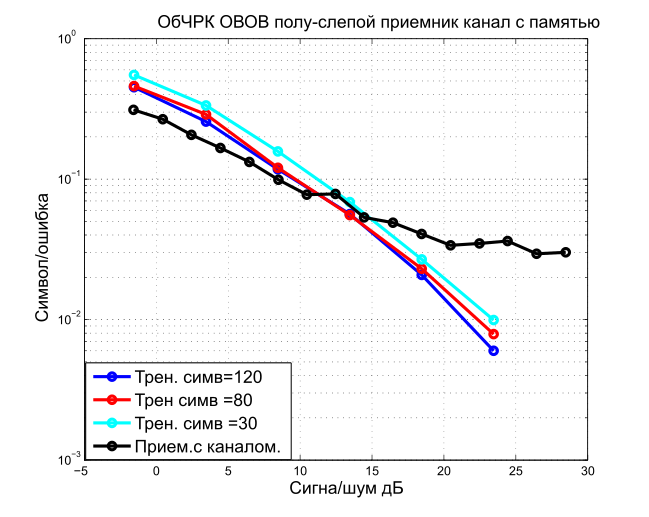
\includegraphics[width=0.9\columnwidth]{SM_SISO_FS_SER.png}
\caption{\textit{Производительность работы полу-слепого приемника от сигнал/шум и количества тренировочных символов}}
\label{fs_8}
\end{figure}
\begin{figure}[H]
\centering
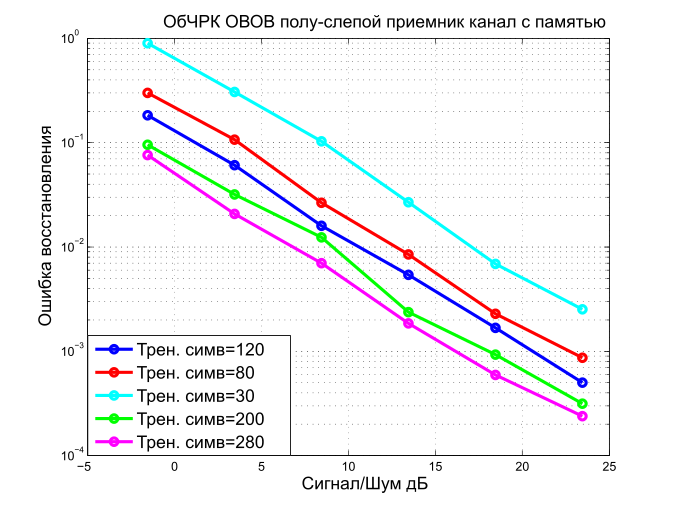
\includegraphics[width=0.9\columnwidth]{SM_SISO_FS_RE.png}
\caption{\textit{Ошибка восстановления канала полу-слепого приемника от сигнал/шум и количества тренировочных символов}}
\label{fs_9}
\end{figure}
\section{Заключение}
Эксперимент по проверке работы полу слепого приемника оценивающего состояние канала и принятые символы показывает следующие результаты:
\begin{itemize}
\item Правильным образом выбирая известные символы в блоке данных можно достичь даже лучшей производительности, чем если идеально знать канал и делать поиск по всем возможным символам.
\item Алгоритм показывает хорошую производительность по каналу пешеходного типа А. 
\item Производительность алгоритма зависит от количества неизвестных символов.
\end{itemize}
Как видно из рис. производительность системы  полу-слепым приемником на основе оптимизации показывает результат лучше, чем даже если был бы использован приемник на основе обратной фильтрации с идеально известным каналом, что говорит о больше стабильности алгоритма. Однако подобное поведение будет изменяться в случае если будут включены только некоторые поднесущие. Производительность системы меняется в зависимости от того сколько символов в блоке данных известно для приемника. После некоторой величины производительность системы падает ниже уровня приемника с идеально известным каналом. Таким образом можно адаптивно регулировать производительность системы. Как видно из рис. кривые ошибки восстановления канала лежат параллельно друг другу позволяя так же адаптивно выбирать точность определения канала гибко, таким образом обновляя состояние канала если он не меняется и уменьшать количество символов на первой итерации для более точного определения канала. Кроме того благодаря использованному подходу с вычитанием известных символов из функции невязки взаимная интерференция между разными каналами так же уменьшается и дополнительно увеличивает производительность системы. Кроме того в случае постановки задачи оптимизации количества излучаемой энергии к количеству полученной информации будет получена вогнутая кривая производительности по качеству работы системы в зависимости от количества известным системе символов.
Основным выводом можно считать что данный подход является чрезвычайно эффективным с точки зрения качества работы системы, однако не является реализуемым на практике с точки зрения оборудования, так как потребует значительных вычислительных ресурсов, однако возможна параллельная обработка принятых данных, что вероятно может ускорить работу системы. Более того для простых задач с небольшими объемами данных современные встроенные системы могут реализовать данные операции.
\clearpage